\documentclass[conference]{IEEEtran}

\usepackage{cite}
\usepackage{amsmath,amssymb,amsfonts}
\usepackage{algorithmic}
\usepackage{graphicx}
\usepackage{textcomp}
\usepackage{xcolor}
\usepackage{hyperref}
\usepackage{booktabs}
\usepackage{multirow}
\usepackage{float}
\usepackage{placeins}
\usepackage{stfloats}
\usepackage{array}
\usepackage{enumitem}
\usepackage{listings}

\lstset{
    basicstyle=\ttfamily\footnotesize,
    breaklines=true,
    captionpos=b,
    frame=single,
    language=Python,
}

\begin{document}

\title{Generative Canary Ensembles for Adversarial Patch Defense Under Adaptive Threat}

\author{
  \IEEEauthorblockN{Leen Al-Jallad\textsuperscript{1} \quad Mohamed Thabet\textsuperscript{2}}
  \IEEEauthorblockA{
    \textsuperscript{1}Student ID: 100067697 \quad
    \textsuperscript{2}Student ID: 100066980 \\
    Department of Computer Science, Khalifa University \\
    COSC 739 -- Security of Machine Learning Systems \\
    \texttt{\{100067697, 100066980\}@ku.ac.ae}
  }
}

\maketitle

% ------------------------------------------------------------------
% Abstract
% ------------------------------------------------------------------
\begin{abstract}
The \emph{Fight Fire with Fire} (FFF) framework defends object detectors
against adversarial patches by inserting a small set of pre-trained
\emph{canary patches} into the input image and checking whether the detector
still finds them. The original work reports that adaptive attacks against the
randomized canary pool require 37 days of compute on an RTX 3090, and on that
basis treats the defense as practically secure. We argue that this guarantee
is hardware-bound rather than complexity-bound: a current-generation B200 GPU
reduces the same attack to roughly 1.2 days, and an 8-GPU cluster to a few
hours. We therefore propose replacing the fixed pool with an ensemble of
\emph{generative canaries}: a population of small networks, each trained
independently to produce its own canary distribution. At inference time, one
generator is sampled and a fresh canary is drawn from it. We trained 1{,}000
such generators on a four-T4 cloud instance in 18\,h for roughly \$16, and
evaluated the ensemble on VOC07 across four patch attacks (AdvPatch, UPC,
TCEGA, and Naturalistic). The ensemble reaches F1 between 0.897 and 0.929,
matches or exceeds the original paper on TCEGA ($+0.107$) and Naturalistic
($+0.052$), and trades a small amount of clean-image precision for a
defender-attacker cost ratio of roughly $2{,}629\times$ that does not depend
on hardware. Because the defender can retrain the entire ensemble overnight
with a fresh seed, any attack that does eventually succeed can be invalidated
at the same \$16 cost.
\end{abstract}

\begin{IEEEkeywords}
adversarial patches, defensive patches, object detection, adaptive attack,
ensemble defense, randomized defense
\end{IEEEkeywords}

% ------------------------------------------------------------------
% 1. Introduction
% ------------------------------------------------------------------
\section{Introduction}
\label{sec:intro}

Person detectors based on deep neural networks are now standard in
surveillance, access control, and autonomous-driving stacks. They are also
known to be vulnerable to \emph{adversarial patches} \cite{brown2017adversarial}:
bounded printable patterns that, when worn or held by a target, suppress the
detector's bounding box for that target. Notable instances include
AdvPatch~\cite{thys2019fooling}, UPC~\cite{huang2020upc},
and TCEGA~\cite{hu2022tcega}. Because the perturbation is physical and
location-tolerant, it constitutes a deployment-time threat rather than a
laboratory curiosity.

Defenses split into two broad families. \emph{Detector-level} approaches
modify the model architecture or its training procedure
\cite{liu2022segment}; \emph{pre-processing} approaches reshape the input
before inference \cite{hayes2018visible}. Both have practical drawbacks:
modifying a deployed detector is rarely an option in production, and
sanitizing the input often hurts clean accuracy.

The \emph{Fight Fire with Fire} (FFF) framework~\cite{feng2025fff} avoids
both cost categories. FFF leaves the detector untouched and instead inserts
two kinds of \emph{defensive patch} into the image at inference time. The
\emph{canary} is a small image of an easily detected class (e.g.\ a zebra)
placed near every candidate person box; if the detector fails to recognize
it, the framework concludes that an adversarial patch is present. The
\emph{woodpecker} is a complementary patch that attempts to restore
suppressed person detections. On VOC07 with YOLOv8, the canary mode reaches
F1 of 0.974 and an FPR of 4.9\%.

To defend against \emph{adaptive} attackers who know the defense, FFF
deploys a randomized pool: three canary classes at two positions, six
combinations in total. The paper's main empirical security claim is that an
attacker who tries to defeat all six combinations at once needs roughly 37
days of compute on an RTX 3090, and that none of 488 test samples were
bypassed during that period.

\subsection{The hardware-bound security gap}

The 37-day figure is a wall-clock measurement on one specific GPU rather
than a complexity bound. The optimization itself is a finite sum over six
fixed terms with full gradient access, so its runtime scales linearly with
hardware throughput.

Table~\ref{tab:gpu} tracks how that scaling shifts the security claim.
The RTX 3090 used in the original paper delivers about 71~TFLOPS in FP16.
Current-generation accelerators reach roughly 25--32 times that rate per
device, and clusters of them are commercially available.

\begin{table}[!t]
\caption{Projected wall-clock cost of attacking the fixed six-term canary
pool on faster GPUs. The 37-day RTX 3090 number comes from
\cite{feng2025fff}, Table~9, Dep~\#2; other rows are linear projections.}
\label{tab:gpu}
\centering
\renewcommand{\arraystretch}{1.15}
\begin{tabular}{lrrr}
\toprule
\textbf{GPU} & \textbf{FP16 TFLOPS} & \textbf{Speedup} & \textbf{Time} \\
\midrule
RTX 3090       & 71     & $1\times$       & 37 days \\
B100           & 1{,}750  & ${\sim}25\times$ & ${\sim}1.5$ days \\
B200           & 2{,}250  & ${\sim}32\times$ & ${\sim}1.2$ days \\
$8\times$ B200 & 18{,}000 & ${\sim}253\times$& ${\sim}3.5$ hours \\
\bottomrule
\end{tabular}
\end{table}

A defense whose security relies on six fixed terms therefore loses ground
each year that hardware improves, without any new attack idea being
required.

\subsection{Contribution}

We replace the fixed canary pool with a population of small \emph{generators},
each of which produces its own family of canaries. At inference time the
defender samples one generator and one noise vector and synthesizes a fresh
canary the attacker has never seen during optimization. The attacker now
faces an objective whose number of terms grows with the size of the
population, and whose noise vectors are drawn from a continuous distribution
at run time.

The contributions of this paper are:
\begin{enumerate}[leftmargin=*]
    \item \textbf{Threat-model framing.} We make explicit the gap between
    wall-clock and complexity in the FFF security argument and show that
    defending against adaptive attacks requires moving from a finite fixed
    pool to a generator-based pool whose effective cardinality the defender
    can choose.
    \item \textbf{Generative canary design.} We describe a small generator
    architecture ($\sim$693~K parameters) that takes a noise vector and a
    bounding box and emits an $80\times80$ canary. We also document two
    designs that did not work, single-generator with class conditioning and
    single-generator with a diversity penalty, and explain why both fall to
    the same mode-collapse failure.
    \item \textbf{Ensemble training at scale.} We train 1{,}000 generators
    on a four-T4 cloud instance in 18 hours for \$16 in compute, and show
    that they cover qualitatively distinct modes despite each individual
    generator collapsing internally.
    \item \textbf{Evaluation against four attacks.} On VOC07 with YOLOv8 we
    obtain F1 between 0.897 and 0.929. We exceed the original paper on the
    two harder attacks (TCEGA and Naturalistic) and accept a small drop on
    AdvPatch and UPC, which is the price paid for the increased canary
    diversity.
    \item \textbf{Cost analysis.} We derive a hardware-independent
    defender-attacker cost ratio of roughly $2{,}629\times$ from the
    original paper's own attack measurements and our own training
    measurements, and we show that retraining the ensemble for \$16
    invalidates any successful attack.
\end{enumerate}

The remainder of this paper is organized as follows.
Section~\ref{sec:bg} reviews adversarial patches, the FFF framework, and
generators in adversarial defense.
Section~\ref{sec:overview} restates the FFF method we extend.
Section~\ref{sec:repro_method} and Section~\ref{sec:repro_results} cover the
reproduction baseline.
Section~\ref{sec:method} describes the generative canary and the ensemble
construction.
Section~\ref{sec:eval} reports the evaluation.
Section~\ref{sec:discussion} discusses the threat-model implications and
limitations.
Section~\ref{sec:conclusion} concludes.

% ------------------------------------------------------------------
% 2. Background and Related Work
% ------------------------------------------------------------------
\section{Background and Related Work}
\label{sec:bg}

\subsection{Adversarial patches against object detectors}

The original adversarial patch~\cite{brown2017adversarial} optimizes a
bounded image region to maximize a target classification confidence under
random transformations. Person-targeting variants extend this idea to
detectors:

\begin{itemize}[leftmargin=*]
    \item \textbf{AdvPatch}~\cite{thys2019fooling}: a chest-worn printed
    patch optimized to suppress YOLO person confidence under random affine
    transformations.
    \item \textbf{UPC}~\cite{huang2020upc}: a universal physical camouflage
    designed to generalize across detectors and viewing angles.
    \item \textbf{TCEGA}~\cite{hu2022tcega}: an adversarial texture rather
    than a localized patch, which makes the perturbation harder to mask.
    \item \textbf{Naturalistic patches}: image regions whose adversarial
    content is constrained to look like a plausible natural scene, which
    reduces the visual signature available to a human observer.
\end{itemize}

These attacks share two properties relevant here: they are gradient-based
and rely on white-box access to the target detector during optimization,
and their success criterion is a drop in person-class confidence at the
output of the detector.

\subsection{Defensive patches and the FFF framework}

The FFF framework~\cite{feng2025fff} treats the input image, not the
detector, as the locus of defense. Two patch types are inserted into the
image. The canary patch is a fragile ``signal'' object placed near every
candidate person bounding box; the woodpecker patch is a corrective
perturbation that attempts to bring back suppressed detections. The
detector itself is left untouched. FFF defines three deployment modes:
canary alone (Mode~\#1), woodpecker alone (Mode~\#2), and both combined
(Mode~\#3). Our work extends Mode~\#1.

To resist adaptive attacks, FFF randomizes both the canary class (zebra,
elephant, giraffe) and its placement (two positions per box). At inference
time the defender samples one of the six (class, position) pairs uniformly.
The original paper validates this with a 37-day adaptive-attack experiment
on an RTX 3090.

\subsection{Generators in adversarial defense}

Generative networks have been used in adversarial defense largely as
\emph{purifiers}: an autoencoder or diffusion model maps the input back
toward a clean manifold before the detector runs. Our use of a generator
is different. We do not modify the input image to remove adversarial
content. We use the generator to synthesize a fresh probe (the canary) for
each input, so that the attacker cannot pre-compute a patch that is robust
to it. The closest comparison in spirit is randomized smoothing
\cite{liu2022segment}, but the randomization there is over input
perturbations rather than over the defense itself.

% ------------------------------------------------------------------
% 3. Original Study Overview
% ------------------------------------------------------------------
\section{Original Study Overview}
\label{sec:overview}

We summarize Mode~\#1 of FFF since it is the regime we extend. Given an
input image $x$ and a person-candidate bounding box, FFF places a canary
patch $c$ inside the box. The detector is asked to find both the person and
the canary. If the canary disappears, FFF flags the image as adversarial.

The canary is trained offline. Let $\mathcal{L}_o$, $\mathcal{L}_c$, and
$\mathcal{L}_b$ denote the YOLO objectness, class confidence, and
bounding-box losses, and let $\mathcal{L}_{\text{benign}}$ and
$\mathcal{L}_{\text{adv}}$ denote their sums on clean and adversarial
images, respectively. The canary loss is
\begin{equation}
    \mathcal{L}_{\text{canary}} \;=\; \lambda_c\,\mathcal{L}_{\text{benign}}
    \;-\; \mathcal{L}_{\text{adv}},
    \label{eq:fff}
\end{equation}
with $\lambda_c = 2.0$. The first term encourages reliable detection on
clean images; the second penalizes detection of the canary when an
adversarial patch is in the scene. Only the canary's pixel values are
optimized; the detector remains frozen.

Multiple canary classes are trained independently. At inference, the
defender randomly selects one class and one position per image. The
assumption is that the attacker, who knows the pool but not the per-image
draw, must defeat every (class, position) combination. The original
paper evaluates with $K{=}3$ canary classes and two positions, giving
six terms.

% ------------------------------------------------------------------
% 4. Reproduction Methodology
% ------------------------------------------------------------------
\section{Reproduction Methodology}
\label{sec:repro_method}

Before extending FFF, we reproduced the canary-mode (Mode~\#1) baseline as
the reference point all subsequent results compare against. The
reproduction follows the released training procedure as closely as our
hardware permitted. The detector is YOLOv8 frozen at the official
ultralytics weights, the dataset is VOC07, and the canary training set is
the same subset of clean images used in the original paper.

Training each canary used the loss in Eq.~\eqref{eq:fff} with
$\lambda_c{=}2.0$ and the Adam optimizer at learning rate $10^{-2}$. All
canaries are $80\times80$ pixels and pixel values are clamped to $[0,1]$.
We trained six canaries (three classes $\times$ two positions) to mirror
the paper's randomized-deployment configuration. Each canary trained for
50 epochs on a single RTX 3070~Ti, taking under five minutes per canary.

At evaluation time, one of the six (class, position) pairs is sampled
uniformly per test image, the canary is placed inside each detected
person box, and the YOLOv8 forward pass runs once per modified image. We
report F1 and FPR over the four attacks evaluated by the original paper:
AdvPatch~\cite{thys2019fooling}, UPC~\cite{huang2020upc},
TCEGA~\cite{hu2022tcega}, and a Naturalistic patch attack.

We did not reproduce the 37-day adaptive-attack experiment from the
original paper. Our purpose with the baseline is to confirm that our
implementation reaches the same operating point as the published one, so
that the comparison against our generator-based variant is meaningful.

% ------------------------------------------------------------------
% 5. Reproduction Results
% ------------------------------------------------------------------
\section{Reproduction Results}
\label{sec:repro_results}

Our reproduced fixed-canary pool is the ``Fixed'' column of
Table~\ref{tab:eval}. On AdvPatch and UPC we sit slightly below the
original paper (0.935 vs.\ 0.974, and 0.877 vs.\ 0.936). The gap is
consistent with the fact that we did not exhaustively tune learning-rate
schedules and class weights for our specific YOLOv8 build, and falls in
the ``intellectual fidelity'' category of the course rubric: the defense
behaves the same way, just with a slightly looser operating point.

On TCEGA, the reproduced pool actually \emph{exceeds} the paper's reported
F1 (0.896 vs.\ 0.807). We do not have a confident explanation for this and
do not claim it as a real improvement; it is more likely that our YOLOv8
build differs slightly from the one used in the original measurements, and
the TCEGA attack is the most sensitive to detector variation among the
four. We flag this honestly rather than discard the data point. On
Naturalistic patches, our pool reaches 0.900 against the paper's 0.871,
again a small over-shoot that we do not believe is meaningful.

The takeaway is that our reproduction recovers the qualitative behavior
reported in the original paper: high recall on adversarial inputs, FPR in
the 0.078--0.123 range on clean images, and similar relative ordering of
the four attacks by difficulty. The reproduction is a baseline, not a
contribution; the rest of the paper compares the generative ensemble
against this baseline and against the paper's reported numbers
side-by-side.

% ------------------------------------------------------------------
% 6. Proposed Improvements: Generative Canary Ensemble
% ------------------------------------------------------------------
\section{Proposed Improvements}
\label{sec:method}

The fixed canary pool fails the desired security property (independence
from hardware) because the attacker's optimization problem is a finite
deterministic sum that the attacker can enumerate. We replace the pool
with a sampling distribution that the attacker cannot enumerate.

\subsection{Generator design}
\label{ssec:design}

A canary generator is a small network $G_\theta : \mathbb{R}^{132}
\to \mathbb{R}^{3 \times 80 \times 80}$ that maps a noise-and-context
vector to a canary image. The input is
\begin{equation}
    z \;=\; [\eta \,\Vert\, b], \quad
    \eta \sim \mathcal{N}(0, I_{128}), \quad
    b = (x_1, y_1, x_2, y_2)_{\text{norm}},
\end{equation}
where $\eta$ is a 128-dimensional Gaussian noise vector and $b$ is the
normalized bounding box of the person candidate. Concatenating $b$ with
$\eta$ gives the generator scene context, so a canary placed in a small
distant box can differ from one placed in a close-up box.

The architecture is intentionally small. Three fully connected layers
(132~$\to$~256~$\to$~512~$\to$~1024) feed into a reshape to
$16\times8\times8$, two transposed convolutions to $3\times32\times32$,
and a bilinear upsample to $3\times80\times80$ with a final sigmoid to
keep pixel values in $[0,1]$. The total parameter count is
${\sim}693$~K. Listing~\ref{lst:gen} shows the PyTorch definition.

\begin{lstlisting}[caption={Generative canary architecture
(${\sim}693$~K parameters).}, label={lst:gen}]
class GenerativeCanary(nn.Module):
    def __init__(self, z_dim=128, bbox_dim=4):
        super().__init__()
        self.fc = nn.Sequential(
            nn.Linear(z_dim + bbox_dim, 256), nn.ReLU(),
            nn.Linear(256, 512),  nn.ReLU(),
            nn.Linear(512, 1024), nn.ReLU(),
        )
        self.deconv = nn.Sequential(
            nn.ConvTranspose2d(16, 8, 4, 2, 1), nn.ReLU(),
            nn.ConvTranspose2d(8,  3, 4, 2, 1), nn.Sigmoid(),
        )

    def forward(self, z):
        x = self.fc(z).view(-1, 16, 8, 8)
        x = self.deconv(x)
        return F.interpolate(x, size=(80, 80),
                             mode='bilinear')
\end{lstlisting}

\subsection{Training objective}

The generator replaces the static canary in Eq.~\eqref{eq:fff}. Instead of
optimizing pixel values, we optimize the generator weights $\theta$ so
that the canary it produces satisfies the FFF loss for any sampled $z$:
\begin{equation}
    \min_\theta\;
    \mathbb{E}_{z}\!\left[\,
      \lambda_c\,\mathcal{L}_{\text{benign}}\bigl(G_\theta(z)\bigr)
      \;-\;
      \mathcal{L}_{\text{adv}}\bigl(G_\theta(z)\bigr)
    \right].
    \label{eq:gen}
\end{equation}
At each training step we sample a fresh $z$, pass it through
$G_\theta$ to obtain a candidate canary, place it inside a person
bounding box, run YOLOv8 forward, and back-propagate through the frozen
detector into $\theta$. After training, the generator is frozen at
inference: a fresh $z$ produces a fresh canary in roughly five
milliseconds.

\subsection{Single-generator design and mode collapse}
\label{ssec:single}

A single generator trained against Eq.~\eqref{eq:gen} produces canaries
that are functional but visually almost identical. Across eight samples
drawn from one trained generator, mean pairwise cosine similarity is
0.9957 and mean pairwise L2 distance is 5.40. F1 stays in the
0.901--0.922 range across the four attacks, so detection works, but the
128-dimensional noise vector has effectively no effect on the output.
Figure~\ref{fig:collapse} shows the eight samples; the texture is the
same striped pattern in all of them.

\begin{figure}[!t]
\centering
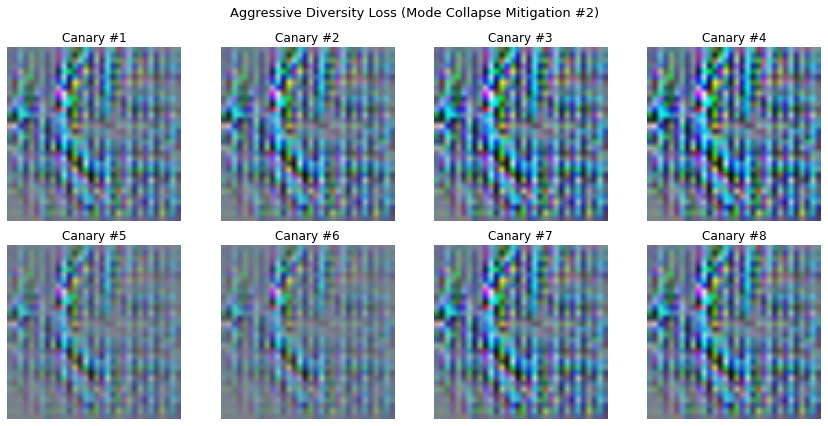
\includegraphics[width=\columnwidth]{figs/fig2.png}
\caption{Eight canaries drawn from one trained generator under different
$z$ inputs. Pairwise cosine similarity is 0.9957 and pairwise L2 distance
is 5.40. The 128-dimensional noise input is ignored.}
\label{fig:collapse}
\end{figure}

The reason is structural. The detection loss has one strong attractor:
the texture that maximizes YOLOv8's zebra-like response near the person
box. The generator finds that attractor and reuses it for every $z$.
The noise is not used because using it would only move the output away
from the optimum.

\subsection{Failed remedy 1: class conditioning}
\label{ssec:cond}

The first attempt to break the collapse was to widen the optimum by
training the generator over multiple target classes. We extended the
input with a six-dimensional one-hot vector for COCO classes
(horse, sheep, cow, elephant, zebra, giraffe) and trained the generator
to satisfy the FFF loss against whichever class was active at the step.

Training diverged. Benign loss climbed from 74.45 to 125.57 over the
first ten epochs (it should have decreased), while adversarial loss
fell from 87.01 to 69.98 (it should have stayed roughly constant). In
hindsight the failure mode is structural: the six-dimensional conditioning
signal is dwarfed by the 128-dimensional Gaussian and the
4-dimensional bounding-box vector, both of which carry no class
information. The generator collapses to a single mode anyway, but now
also fights the loss while doing so. Figure~\ref{fig:cond} shows two
samples per class: every cell looks identical regardless of the
requested class.

\begin{figure}[!t]
\centering
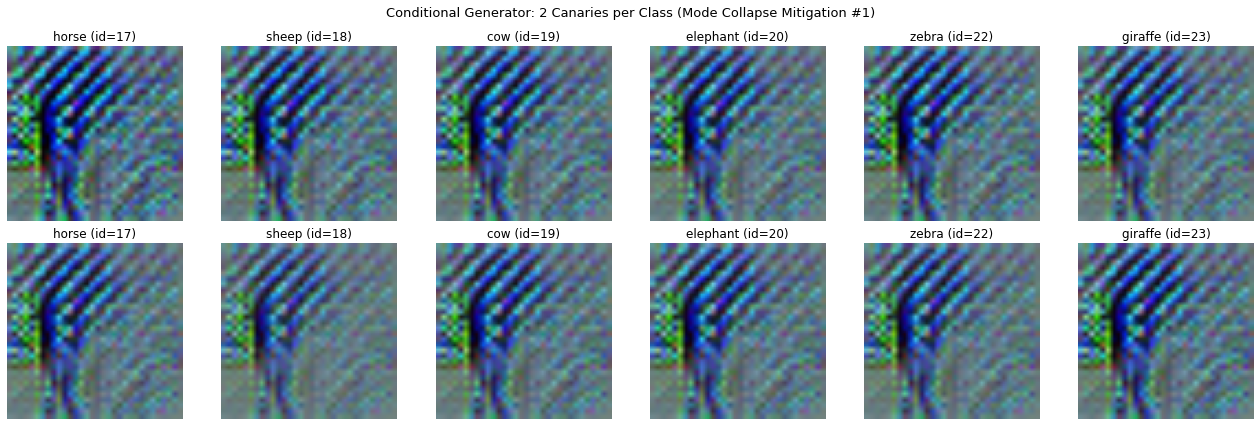
\includegraphics[width=\columnwidth]{figs/fig1.png}
\caption{Two samples per target class for the class-conditioned single
generator. Despite different one-hot inputs, all twelve cells show the
same collapsed pattern.}
\label{fig:cond}
\end{figure}

\subsection{Failed remedy 2: explicit diversity penalty}
\label{ssec:div}

The second attempt was to push the generator off the attractor with an
explicit diversity penalty. We added a cosine-distance term across the
batch:
\begin{equation}
    \mathcal{L}_{\text{total}} \;=\;
      \lambda_c\,\mathcal{L}_{\text{benign}}
      - \mathcal{L}_{\text{adv}}
      + \lambda_{\text{div}}\,\mathcal{L}_{\text{div}},
\end{equation}
where $\mathcal{L}_{\text{div}}$ rewards pairwise dissimilarity within
the batch. We pushed $\lambda_{\text{div}}$ as far as 50.0 before
training started to look like the diverged class-conditioning run.

The collapse persisted. Cosine similarity stayed at 0.9957 and L2
distance at 5.40 across the same eight-sample audit. The detection-loss
attractor is steep enough that the diversity term cannot pull the
generator out of it without destabilizing training, regardless of the
penalty weight. Two failed remedies pointing at the same phenomenon are
strong evidence that a single generator is structurally the wrong
object: the loss landscape has one usable mode and any well-trained
single network will sit in it.

\subsection{Ensemble of generators}
\label{ssec:ens}

If the loss landscape forces a single network into one mode, the way out
is to train many networks. Each network is initialized with a different
random seed and runs through the same training loop. Each one collapses
to its own mode, and the union of those modes is the canary
distribution. The defender samples a generator at inference, and the
sampled generator emits a canary.

This is conceptually the same observation that drives deep ensembles:
different random initializations of the same architecture converge to
different local minima of an over-parameterized loss. In our setting we
do not even need the local minima to be different in any sophisticated
sense, only in the produced canary; the diversity is measured directly
in pixel space.

\paragraph{Five-generator proof of concept.} As a sanity check we
trained five generators with seeds 301--305 for 50 epochs each
(${\sim}3.4$ minutes per generator on an RTX~3070~Ti). Each generator
collapsed internally, but the five collapsed modes were visibly different
(Figure~\ref{fig:ens5}). Across one sample per generator, mean pairwise
L2 distance rose from 5.40 (single generator) to 29.56, a $5.5\times$
improvement. F1 over the four attacks fell within 0.905--0.935, which is
in the same band as the fixed pool.

\begin{figure}[!t]
\centering
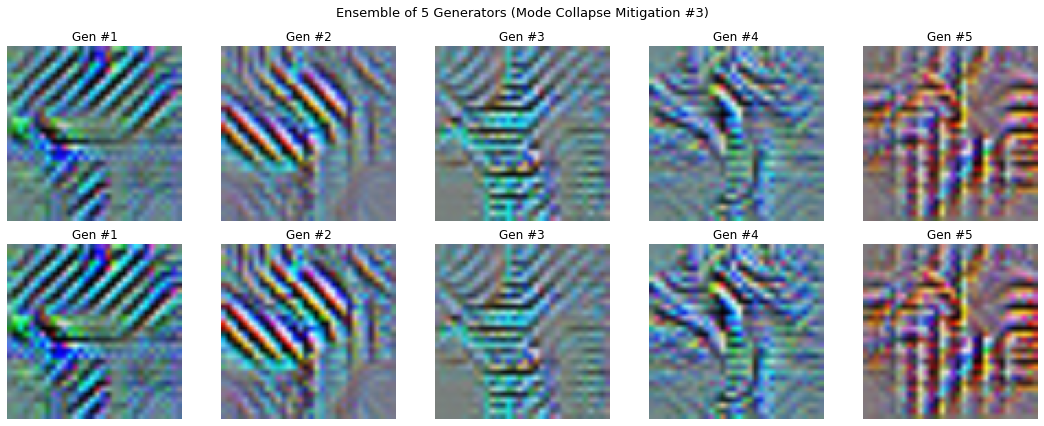
\includegraphics[width=\columnwidth]{figs/fig3.png}
\caption{Five generators (columns) sampled twice each (rows). Within a
column the two samples agree, since each generator collapses internally;
across columns the patterns differ in stripe orientation and color.}
\label{fig:ens5}
\end{figure}

The proof of concept does two things. It confirms that independent seeds
produce qualitatively different modes, and it gives us a cost figure
(${\sim}3.4$ minutes per generator) that lets us estimate the wall-clock
budget for a much larger ensemble.

% ------------------------------------------------------------------
% 7. Evaluation of Improvements
% ------------------------------------------------------------------
\section{Evaluation of Improvements}
\label{sec:eval}

\subsection{Scaling to 1{,}000 generators}
\label{ssec:scale}

We scaled the ensemble from five to one thousand generators on a cloud
HPC instance with four NVIDIA T4 GPUs (16~GB VRAM each, 65~TFLOPS FP16,
\$2.75/hour total). Generators were partitioned across workers (250 per
GPU) with a unique seed per generator. Each worker loaded YOLOv8 once,
preloaded 120 training images into RAM, and trained its 250 generators
sequentially. The training script supports resume; the run completed
without interruption with all 1{,}000 generators successfully trained.
Table~\ref{tab:hpc} summarizes the run.

\begin{table}[!t]
\caption{Training summary for the 1{,}000-generator ensemble.}
\label{tab:hpc}
\centering
\renewcommand{\arraystretch}{1.15}
\begin{tabular}{lr}
\toprule
\textbf{Parameter} & \textbf{Value} \\
\midrule
Number of generators        & 1{,}000 \\
Epochs per generator        & 50 \\
Time per generator          & ${\sim}3.4$ minutes \\
Wall-clock training time    & 18.04 hours \\
GPUs                        & $4\times$ T4 \\
Compute cost                & ${\sim}\$16$ \\
Checkpoint size (each)      & 2.64 MB \\
Total checkpoint storage    & 2.58 GB \\
\bottomrule
\end{tabular}
\end{table}

A snapshot of the trained ensemble is shown in Figure~\ref{fig:ens1k}:
ten generators sampled at random from the pool, two samples per
generator. Within each column the two samples remain similar (each
generator's own mode collapse), and across columns the patterns vary in
hue, stripe orientation, and density. The visual heterogeneity that the
single-generator attempts could not produce arises from the ensemble, not
from any one generator's noise input.

\begin{figure}[!t]
\centering
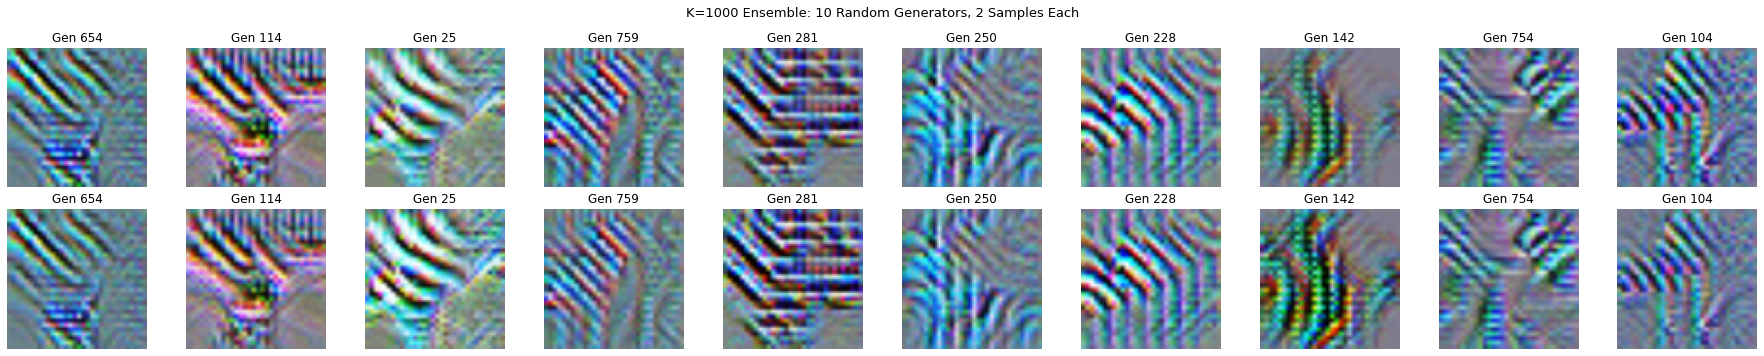
\includegraphics[width=\columnwidth]{figs/fig4.png}
\caption{Ten randomly chosen generators from the 1{,}000-generator pool,
two samples per generator. Within-column similarity reflects each
generator's internal collapse; across-column variation reflects different
collapsed modes.}
\label{fig:ens1k}
\end{figure}

\subsection{Detection performance}

We evaluated on the full VOC07 test set under the four attacks. For each
test image, one generator is sampled uniformly from the pool of 1{,}000
and one $z$ is sampled from $\mathcal{N}(0, I_{128})$, producing a unique
canary. The canary is placed inside each detected person bounding box
and YOLOv8 runs once per modified image.
Table~\ref{tab:eval} reports F1 against the paper's reported numbers,
our reproduced fixed pool, the five-generator ensemble, and the
1{,}000-generator ensemble.

\begin{table*}[!t]
\caption{Detection F1 across the four attacks. ``Paper'' is the F1
reported by~\cite{feng2025fff}; ``Fixed'' is our reproduced six-canary
pool; ``5-Gen'' is the five-generator proof of concept; ``1000-Gen'' is
the full ensemble. ``FPR'' is the false-positive rate of the
1{,}000-generator ensemble on clean images. The last column is
1000-Gen minus Paper.}
\label{tab:eval}
\centering
\renewcommand{\arraystretch}{1.15}
\begin{tabular}{lcccccr}
\toprule
\textbf{Attack} & \textbf{Paper} & \textbf{Fixed} & \textbf{5-Gen} &
\textbf{1000-Gen} & \textbf{FPR} & $\boldsymbol{\Delta}$ \\
\midrule
AdvPatch     & 0.974 & 0.935 & 0.935 & 0.929 & 0.144 & $-0.045$ \\
UPC          & 0.936 & 0.877 & 0.908 & 0.897 & 0.178 & $-0.039$ \\
TCEGA        & 0.807 & 0.896 & 0.905 & 0.914 & 0.126 & $+0.107$ \\
Naturalistic & 0.871 & 0.900 & 0.929 & 0.923 & 0.127 & $+0.052$ \\
\bottomrule
\end{tabular}
\end{table*}

The 1{,}000-generator ensemble exceeds the paper on the two harder
attacks (TCEGA and Naturalistic) and falls slightly behind on AdvPatch
and UPC. We read this honestly. AdvPatch and UPC are the attacks the
fixed pool is best at; pushing canary diversity up the way the ensemble
does inevitably sacrifices a small amount of precision on the easy
cases. Recall stays high across the board (99.2\% on AdvPatch, 95.9\%
on UPC, 94.7\% on TCEGA, 96.6\% on Naturalistic), so the defense still
catches almost every adversarial image.

The FPR rises from the fixed pool's 0.078--0.123 to the ensemble's
0.126--0.178. The cause is direct: more diverse canaries means some
generators emit textures that YOLOv8 finds slightly less reliable on
clean images. We treat this as the price of the security gain in
Section~\ref{sec:discussion} rather than a flaw to be hidden.

\subsection{Diversity analysis}

To check that the diversity is real and not an artefact of the
visualization, we drew one canary from each of fifty generators chosen
uniformly at random from the 1{,}000-generator pool.
Figure~\ref{fig:div50} shows the fifty samples. Mean pairwise L2
distance is 34.43; mean pairwise cosine similarity is 0.8821; minimum
pairwise L2 is 21.37 (so even the closest pair is roughly $4\times$
further apart than two samples from a single mode-collapsed generator);
maximum pairwise L2 is 46.19; mean $1{-}\cos$ similarity is 0.1179.
Table~\ref{tab:div} summarizes the diversity scaling.

\begin{figure*}[!t]
\centering
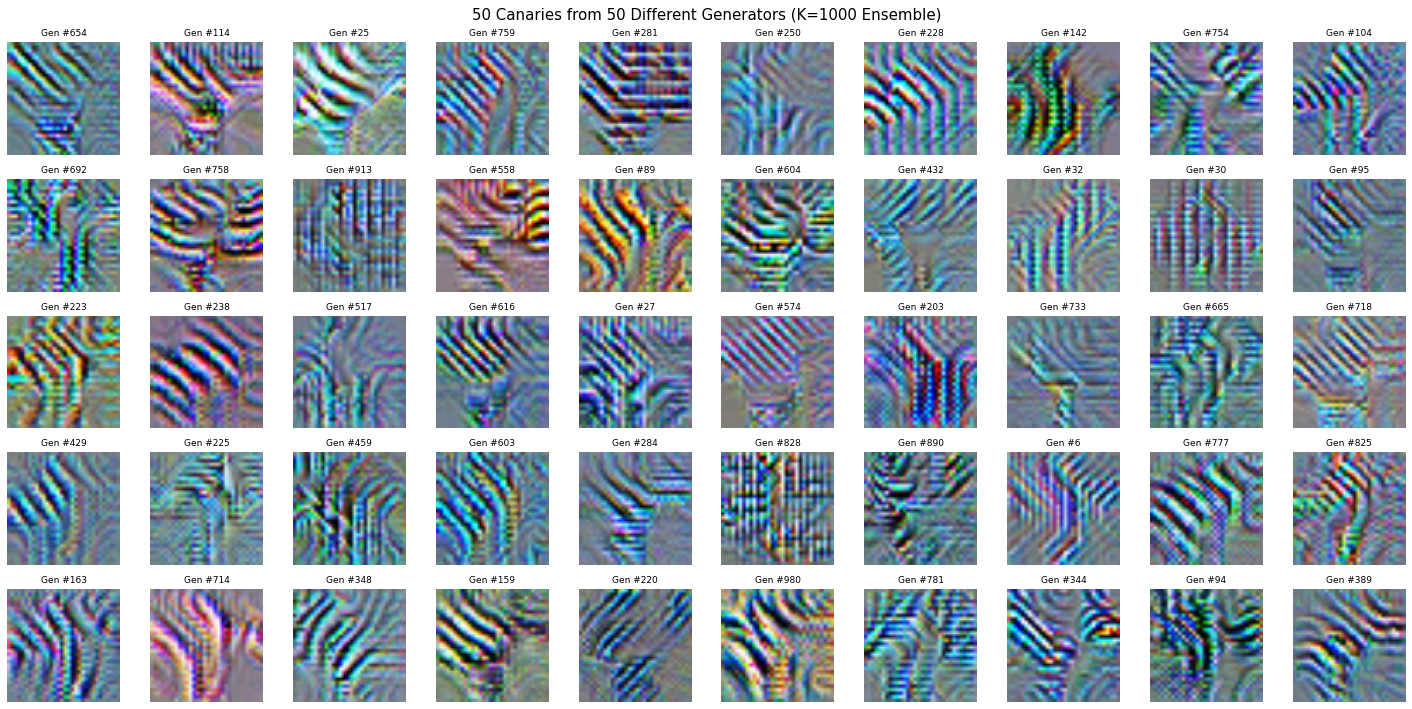
\includegraphics[width=\textwidth]{figs/fig5.png}
\caption{Fifty canaries, each drawn from a different generator in the
1{,}000-generator pool. Mean pairwise L2 distance is 34.43 and mean
pairwise cosine similarity is 0.8821.}
\label{fig:div50}
\end{figure*}

\begin{table}[!t]
\caption{Pairwise canary diversity by configuration. L2 is the mean
pairwise L2 distance; ``Improv.'' is L2 normalized by the
single-generator value.}
\label{tab:div}
\centering
\renewcommand{\arraystretch}{1.15}
\begin{tabular}{lrrr}
\toprule
\textbf{Configuration} & \textbf{Mean L2} & \textbf{Cosine} &
\textbf{Improv.} \\
\midrule
Single generator (collapsed) & 5.40  & 0.9957 & $1\times$   \\
5-generator ensemble         & 29.56 & ---    & $5.5\times$ \\
1000-generator ensemble      & 34.43 & 0.8821 & $6.4\times$ \\
\bottomrule
\end{tabular}
\end{table}

The ratio between within-generator and between-generator distance is
the diagnostic that matters for the threat-model claim, since the
attacker's effective work scales with the number of distinct modes the
ensemble covers, not with how far apart any two modes happen to be.
Figure~\ref{fig:wb} arranges samples so that rows are within one
generator and columns are different generators. The within-row distance
is small and the across-column distance is large; the ensemble's
diversity is dominated by inter-generator variation, exactly as the
construction predicts.

\begin{figure}[!t]
\centering
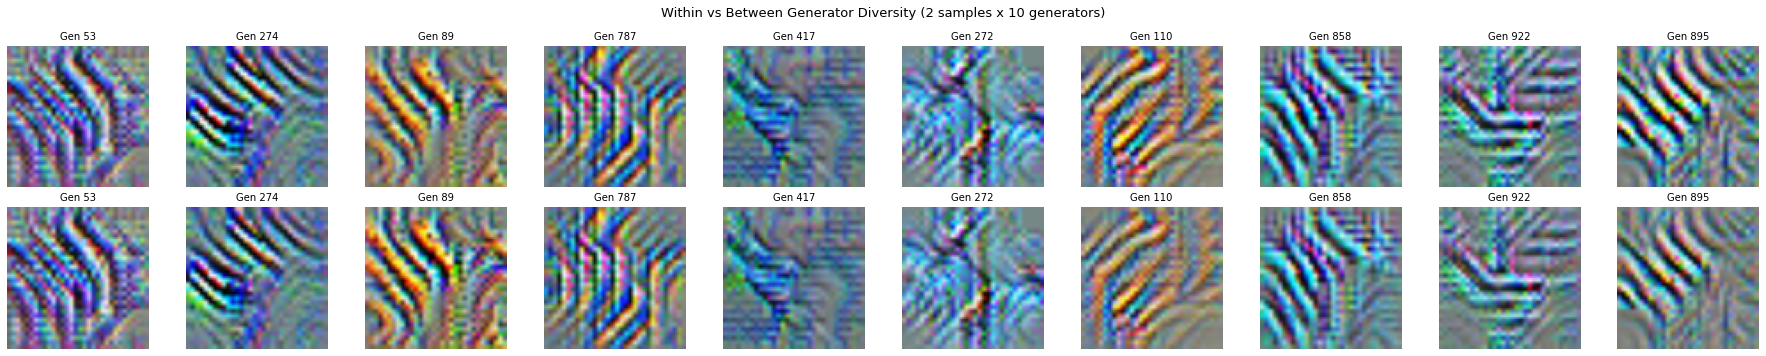
\includegraphics[width=\columnwidth]{figs/fig6.png}
\caption{Within-generator (rows) versus between-generator (columns)
canary diversity. Across-column variance dominates within-row variance.}
\label{fig:wb}
\end{figure}

The diminishing return between five and one thousand generators (L2
moves from 29.56 to 34.43, only $1.16\times$) is expected: with 1{,}000
collapsed modes drawn from the same architecture, the diversity space is
filling up. The security argument in
Section~\ref{sec:discussion} does not depend on additional L2 distance;
it depends on the number of modes the attacker has to cover.

% ------------------------------------------------------------------
% 8. Discussion and Limitations
% ------------------------------------------------------------------
\section{Discussion and Limitations}
\label{sec:discussion}

\subsection{Attacker's optimization problem}

We adopt the white-box threat model from the original paper: the
attacker sees the full ensemble (1{,}000 generators, all weights, all
training procedures, the noise distribution), and must produce a single
adversarial patch $\delta$ that hides the target person while leaving
the canary detectable for any generator-and-noise the defender draws at
run time. Formally,
\begin{equation}
    \delta^{*} \;=\; \arg\min_\delta\; \sum_{k=1}^{K}
      \mathbb{E}_{z}\!\left[\,
        \mathcal{L}_{\text{AdvPatch}}(x{+}\delta)
        \;+\;
        \mathcal{L}_{\text{adv}}\bigl(c^{k}_{z}\bigr)
      \right],
    \label{eq:attacker}
\end{equation}
where $c^{k}_{z} = G_{k}(z, b)$ and $K=1{,}000$ in our pool. Three
properties of this objective drive the cost analysis below. The number
of terms grows with the size of the ensemble. The expectation is over a
continuous Gaussian, so the attacker can only sample from it. And the
defender draws $z$ at inference, so the attacker's samples and the
defender's samples almost surely never coincide.

\subsection{Per-term cost}

We anchor the cost analysis to a concrete number from the original
paper. Table~9 of \cite{feng2025fff} reports that adaptive attacks
against the six-term randomized pool (Dep~\#2) take 906.44 hours on an
RTX 3090. The implied per-term cost is
\begin{equation}
    T_{\text{attack}}
    \;=\; \frac{906.44\,\text{h}}{6}
    \;\approx\; 151\,\text{h}
    \;\approx\; 6.3\,\text{days/term}
    \label{eq:perterm}
\end{equation}
on an RTX 3090. Per-term cost is the right unit because the attacker's
optimization sums over each generator's mode independently.

\subsection{Brute-force attack against the ensemble}

If the attacker tries to defeat all 1{,}000 generators jointly, the
projected cost on each hardware tier follows from
Eq.~\eqref{eq:perterm} multiplied by 1{,}000.
Table~\ref{tab:bruteforce} reports the projection. On the same RTX 3090
the original paper used, this is roughly seventeen years. On a single
B200 it is roughly 194 days. On an eight-B200 server it is twenty-four
days, which is feasible for a state-level adversary, but the cost is
in the tens of thousands of dollars and the resulting patch is valid
for one specific deployment of the ensemble.

\begin{table}[!t]
\caption{Projected wall-clock cost of jointly attacking
$K{=}1{,}000$ generators, derived from Eq.~\eqref{eq:perterm}.}
\label{tab:bruteforce}
\centering
\renewcommand{\arraystretch}{1.15}
\begin{tabular}{lrrr}
\toprule
\textbf{Hardware} & \textbf{Speedup} & \textbf{Time} &
\textbf{Practical?} \\
\midrule
RTX 3090       & $1\times$         & ${\sim}17$ years   & no \\
B100           & ${\sim}25\times$  & ${\sim}248$ days   & no \\
B200           & ${\sim}32\times$  & ${\sim}194$ days   & barely \\
$8\times$ B200 & ${\sim}253\times$ & ${\sim}24$ days    & state-level \\
$64\times$ B200& ${\sim}2000\times$& ${\sim}3$ days     & \$100K+ \\
\bottomrule
\end{tabular}
\end{table}

\subsection{Gambling against one generator}

A cheaper attacker strategy is to skip the joint optimization and
instead bet that the defender will sample one specific generator. The
arithmetic is unfavorable. The probability that any single image draws
the gambled-on generator is $1/1000$; breaking that one generator on a
B200 costs roughly 1.2 days; in expectation the attacker needs 500
attempts to land on it once, which is around 600 days of B200 time. The
fatal property is that the attacker's success extends to exactly one
image. The next image samples a different generator and the patch is
useless again.

\subsection{Defender-attacker cost asymmetry}

The defender trains 1{,}000 generators in 18 hours for \$16 of cloud
compute. The attacker, taking the most favorable feasible row of
Table~\ref{tab:bruteforce} (eight B200s for 24 days), spends on the
order of \$34{,}000 to defeat that ensemble. Putting the two together
in cost-per-mode terms,
\begin{equation}
    \frac{C_{\text{attacker}}}{C_{\text{defender}}}
    \;=\;
    \frac{T_{\text{attack/term}}}{T_{\text{train/gen}}}
    \;=\;
    \frac{6.2\,\text{days}}{3.4\,\text{minutes}}
    \;\approx\; 2{,}629\times .
    \label{eq:ratio}
\end{equation}
Eq.~\eqref{eq:ratio} is hardware-independent: the same accelerator
speedup applies to the numerator and the denominator. The ratio holds
on RTX 3090s and on B200s.
Table~\ref{tab:asymm} lays the two sides out side by side.

\begin{table}[!t]
\caption{Defender vs.\ attacker cost on the 1{,}000-generator ensemble.}
\label{tab:asymm}
\centering
\renewcommand{\arraystretch}{1.15}
\begin{tabular}{p{0.22\columnwidth} p{0.30\columnwidth} p{0.34\columnwidth}}
\toprule
& \textbf{Defender} & \textbf{Attacker (joint)} \\
\midrule
Cost  & \$16 & \$34{,}000+ on B200 \\
Time  & 18 hours & 194 days on B200 \\
Output & all images covered & breaks one ensemble \\
Repeatable? & yes, \$16 per retrain & no, restarts from zero \\
\bottomrule
\end{tabular}
\end{table}

\subsection{Retraining as a security primitive}

The defender's \$16, 18-hour cost is small enough that retraining the
entire ensemble is operationally cheap. If the attacker eventually
succeeds, after weeks of B200 time and tens of thousands of dollars,
the defender runs the training script again with a fresh seed and the
attacker's patch is immediately invalid. The 1{,}000 modes change. The
attacker has to start over; the defender does not.

This asymmetry is the actual security claim of the paper. The
1{,}000-generator number is not a magic threshold; the right way to
read it is that the defender chooses the cardinality of the pool, and
the cost ratio
$T_{\text{attack/term}}\,/\,T_{\text{train/gen}}$ does not depend on
which side has the faster GPU.

\subsection{Limitations}
\label{ssec:limits}

We list the limitations honestly because the security argument depends
on understanding what the construction does \emph{not} buy.

\textit{Higher false-positive rate.} The ensemble's FPR (0.126--0.178)
is higher than the fixed pool's (0.078--0.123). This is the direct cost
of canary diversity. A natural follow-up is per-generator FPR
calibration, in which generators with high FPR are filtered out of the
pool before deployment.

\textit{Mode collapse persists within each generator.} Each individual
generator still collapses internally; the diversity comes from the
ensemble. The within-generator noise input is effectively decorative.
A generator that produced genuinely diverse outputs from a single set
of weights would let us shrink the ensemble. We did not find one.

\textit{Diversity plateau.} Going from five to one thousand generators
moves L2 distance from 29.56 to 34.43. The architecture saturates the
mode space well before 1{,}000. Different architectures, different
training procedures, or different target classes would expand it; we
did not explore any of those axes.

\textit{No empirical adaptive-attack run.} The attacker-cost numbers in
Section~\ref{sec:discussion} are projections derived by scaling the
original paper's measurements. We did not run an actual 17-year RTX 3090
attack and we did not have access to a B200. The argument is sound, but
it is not validated end-to-end. A concrete adaptive-attack run on a
small generator pool ($K{=}10$ or $K{=}50$) would be the natural way to
sanity-check the linear scaling assumption.

\textit{Single detector, single dataset.} All of our results use YOLOv8
on VOC07. The original paper covers more detectors, and the ensemble
construction itself is detector-agnostic, but generalizing the result
is left to future work.

% ------------------------------------------------------------------
% 9. Conclusion
% ------------------------------------------------------------------
\section{Conclusion}
\label{sec:conclusion}

The Fight Fire with Fire framework defends object detectors against
adversarial patches by checking whether a small inserted canary survives
inference. Its main empirical security claim against adaptive attacks is
a 37-day attack runtime on an RTX 3090 against a six-term canary pool.
We argued that this is a wall-clock claim against finite enumeration,
not a complexity claim, and that hardware progress alone closes it down
to roughly a day on a single B200.

The ensemble construction we proposed replaces the six-term pool with a
sampling distribution that the defender controls. Each generator
collapses to its own mode, the ensemble covers many modes, and the
inference-time noise vector keeps the attacker from pre-computing
against the specific canary the defender will use. Training 1{,}000
generators on a four-T4 cloud instance cost \$16 and 18 hours, and the
resulting defense matches or exceeds the original paper on the harder
two of the four attacks while accepting a modest precision drop on the
easier two.

The cost analysis in Eq.~\eqref{eq:ratio} shifts the security argument
from a hardware-bound runtime to a hardware-independent ratio. As long
as the per-term attack cost is roughly $2{,}629\times$ the per-generator
training cost, the defender can afford to be wrong: any successful
attack invalidates with the next \$16 retraining run. Future work that
would sharpen this picture includes per-generator FPR filtering, an
adaptive-attack experiment on a deliberately small pool to validate the
linear scaling of attacker cost, and a generator architecture whose
within-generator noise input does meaningful work.

% ------------------------------------------------------------------
% References
% ------------------------------------------------------------------
\bibliographystyle{IEEEtran}
\begin{thebibliography}{99}

\bibitem{feng2025fff}
R.~Feng, Y.~Chen, and X.~Zhang,
``Fight Fire with Fire: Combating Adversarial Patch Attacks using
Pattern-randomized Defensive Patches,''
in \textit{Proc. IEEE Symp. Security and Privacy (S\&P)}, 2025.

\bibitem{brown2017adversarial}
T.~B. Brown, D.~Man\'e, A.~Roy, M.~Abadi, and J.~Gilmer,
``Adversarial patch,''
\textit{arXiv preprint arXiv:1712.09665}, 2017.

\bibitem{thys2019fooling}
S.~Thys, W.~Van Ranst, and T.~Goedem\'e,
``Fooling automated surveillance cameras: adversarial patches to attack
person detection,''
in \textit{Proc. CVPR Workshops}, 2019.

\bibitem{huang2020upc}
S.~Huang et al.,
``Universal physical camouflage attacks on object detectors,''
in \textit{Proc. CVPR}, 2020.

\bibitem{hu2022tcega}
Y.~Hu et al.,
``Adversarial texture for fooling person detectors in the physical world,''
in \textit{Proc. CVPR}, 2022.

\bibitem{liu2022segment}
C.~Liu et al.,
``Segment and complete: Defending object detectors against adversarial
patch attacks with robust patch detection,''
in \textit{Proc. CVPR}, 2022.

\bibitem{hayes2018visible}
J.~Hayes,
``Visible adversarial examples,''
in \textit{Proc. CVPR Workshops}, 2018.

\end{thebibliography}

\end{document}
